\documentclass[titlepage]{article}
\usepackage{graphicx}
\usepackage{fancyhdr}
\usepackage{hyperref}
\usepackage{tabularx}
\usepackage{multicol}

\title{Client Interaction Report Set}
\author{
	Andrew Borba\\ \emph{Prototyper}	\and
	 Lizz Brooks\\ \emph{Project Manager}	\and
	 Jorge Go\\ \emph{Feasability Analyst}	\and
	 Katherine Hu\\ \emph{Lifecycle Planner}	\and
	 Nakul Joshi\\ \emph{Software Architect}	\and
	 Ian Malave\\ \emph{Requirements Engineer}	\and
	 Rishi Mukhopadyay\\ \emph{Operational Concept Engineer}
}
\date{September 16\textsuperscript{th}, 2013}

\begin{document}
\pagestyle{fancy}
\lhead{Client Interaction Report Set}
\chead{}
\rhead{Version 1.0.1}
\lfoot{}
\cfoot{\thepage}
\rfoot{}

\maketitle
\tableofcontents
\newpage
\section{Version History}
\begin{table}[h]
	\centering
    \begin{tabularx}{\textwidth}{lllXX}
    	\hline
        Date       & Author & Version & Changes Made                                         & Rationale                    \\ \hline
        08/20/2013 & SK     & 1.0     & Original for CS 477; Tailored from ICSM REQ Template & To fit CS 477 Course Content \\ 
        09/14/2013 & Team 1 & 1.0.1   & First version                                                   & Project Requirements                          \\
		\hline
    \end{tabularx}
\end{table}
\newpage
\section{Client Interaction Report}
\newpage


\subsection{Shared Vision}

	\subsubsection{System Overview}\begin{multicols}{2}
				\paragraph{Key Partners}\begin{enumerate}
			\item LA Metro
		\end{enumerate}
		
		\paragraph{Key Activities}\begin{enumerate}
			\item Software Design and Development
			\item Integration with Metro  infrastructure
			\item Marketing of application
		\end{enumerate}
		
		\paragraph{Key Resources}\begin{enumerate}
			\item Development Team
			\item PhoneGap API
			\item NFC technology
			\item QR technology
		\end{enumerate}
		
		\paragraph{Value Proposition}\begin{enumerate}
			\item Convenience for customers to purchase and use metro tickets
			\item Ticket elimination reducing cost and environmental impact
			\item Technological advancement of public transportation system. 
 		\end{enumerate}
 		
 		\paragraph{Customer Relation}\begin{enumerate}
 			\item LA Metro
 			\item Apple Appstore
 			\item Android Store
 			\item Windows Phone Marketplace
 		\end{enumerate}

 		\paragraph{Channels}\begin{enumerate}
 			\item Application stores
 			\item LA Metro website
 			\item Posters and billboards at stations. 
 		\end{enumerate}
 		
 		\paragraph{Customer Segments}\begin{enumerate}
 			\item Transportation Companies
 		\end{enumerate}
 		
 		\paragraph{Cost Structure}\begin{enumerate}
 			\item Development Team
 			\item Back-end System Administrator
 		\end{enumerate}
 		
 		\paragraph{Revenue Streams}\begin{enumerate}
 			\item Flat fee for project implementation
 			\item Recurring fee per ticket sale through application
 		\end{enumerate}
	\end{multicols}
 	\newpage

 	\subsubsection{System Boundary and Environment}
 	\begin{figure}[h]
 		\centering
 		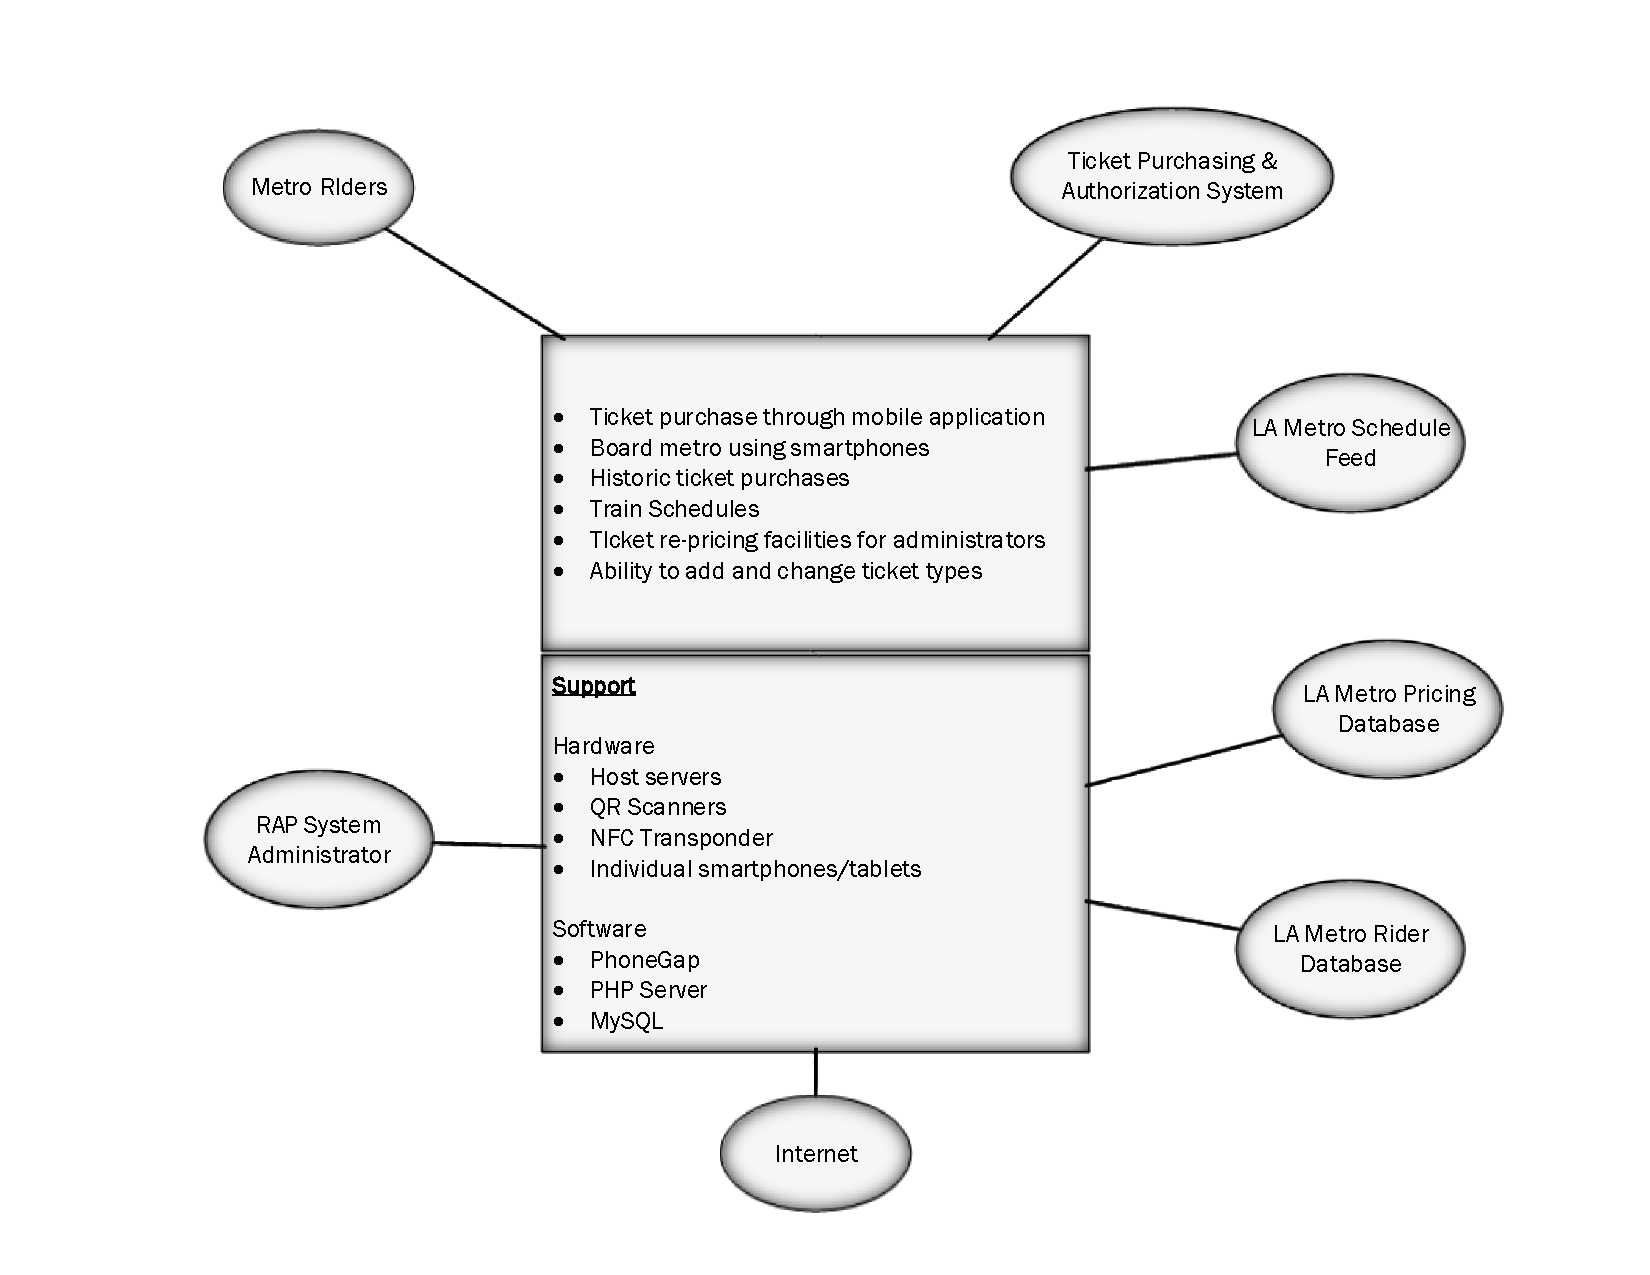
\includegraphics[width=\textwidth]{OCD/boundary.pdf}
 	\end{figure}
 	\newpage
 		
\subsection{System Transformation}
	\subsubsection{System Objectives, Constraints, and Priorities}
		

% Booktabs require to add \usepackage{booktabs} to your document preamble
\begin{table}[h]
\begin{tabularx}{\textwidth}{Xl}
\toprule
Capability Goals                                                                             & Priority Level                                                           \\ \midrule
\textbf{OC-1} Cross-platform Compatible:                                                              & Must have                                                                \\
\multicolumn{2}{X}{The application is compatible with iOS, Android and Windows Phone}                                                                                   \\
\textbf{OC-2} Account Creation:                                                                       & Must have                                                                \\
\multicolumn{2}{X}{The application is able to create new rider accounts, update information, and log in users using existing information.}                              \\
\textbf{OC-3} Usage:                                                                                  & Must have                                                                \\
\multicolumn{2}{X}{The application allows metro riders to board trains via NFC or QR code technology.}                                                                  \\
\textbf{OC-4} Payments:                                                                               & Must have                                                                \\
\multicolumn{2}{X}{The application allows metro riders to pay for tickets using a secure payment gateway and will allow metro riders to store credit card information.} \\
\textbf{OC-5} Schedules:                                                                              & Should have                                                              \\
\multicolumn{2}{X}{The application allows metro riders to view train schedules.}                                                                                        \\
\textbf{OC-6} Map:                                                                                    & Should Have                                                              \\
\multicolumn{2}{X}{The application allows metro riders to view a static map of metro stations.}                                                                         \\
\textbf{OC-7} Updates:                                                                                & Should Have                                                              \\
\multicolumn{2}{X}{The application allows metro riders to receive updates about train station information and irregular service interruptions.}                         \\
\textbf{OC-8} Pricing:                                                                                & Should Have                                                              \\
\multicolumn{2}{X}{The administration application will allow metro administrators to change ticket pricing.}                                                            \\
\textbf{OC-9} Ticket Types:                                                                           & Could Have                                                               \\
\multicolumn{2}{X}{The application will support linking of additional tap accounts for the purpose of allowing dependants to be charged with one QR scan.}              \\
\textbf{OC-10} Ticket Display:                                                                        & Should Have                                                              \\
\multicolumn{2}{X}{The application will use GPS services to automatically display tickets for the closest station.}           \\
\bottomrule                                         
\end{tabularx}
\end{table}

% Booktabs require to add \usepackage{booktabs} to your document preamble
\begin{table}[h]
\centering
\begin{tabular}{@{}ll@{}}
\toprule
Level of Service Goals     & Priority Level \\ \midrule
Reliability of application & Must have      \\
Usability                  & Must have      \\
Security                   & Must have      \\
Performance of system      & Should have    \\
Inter-operability          & Should have    \\
Maintainability            & Should have   \\
\bottomrule
\end{tabular}
\end{table}


\paragraph{Organizational Goals}\begin{description}
	\item[OG-1] Increase convenience for ticket buyers.
	\item[OG-2] Decrease cost for LA Metro and ticket buyers. 
	\item[OG-3] Increase efficiency of public transit system by advancing technologically.
\end{description}

\paragraph{Constraints}\begin{description}
	\item[CO-1] Align with Current Infrastructure: The new application must complement the existing tap card system, and be implemented with minimal changes to existing infrastructure. 
	\item[CO-2] Cross Platform Compatibility: The new application must be compatible with major smartphone operating systems(iOS, Android and Windows)
	\item[CO-3] Phone Hardware: The application must be compatible with the existing hardware in major smartphones.

\end{description}
	
	
	\subsubsection{Proposed Operational Concept}
		The application will allow metro riders to use their mobile devices to purchase tickets and board trains eliminating the need for physical TAP cards. The new system will act as a complement to the TAP card system; allowing riders to use existing metro facilities if they wish.
		
		For those smartphones enabled with NFC, the rider will be able to “tap” their phones instead of their tap cards. For those smartphones not enable with NFC, QR readers will be installed at stations that have turnstiles. For stations that do not have turnstiles, Metro agents will be given a QR reader to verify tickets on the train.
		
	The application will allow users to view train schedules along with a map of the stations in the users’ metro system. Users will also receive news updates in case of unusual delays or train cancellations. 
	
\clearpage
	\subsubsection{Proposed Element Relationship}
		\begin{figure}[!htbp]
			\centering
				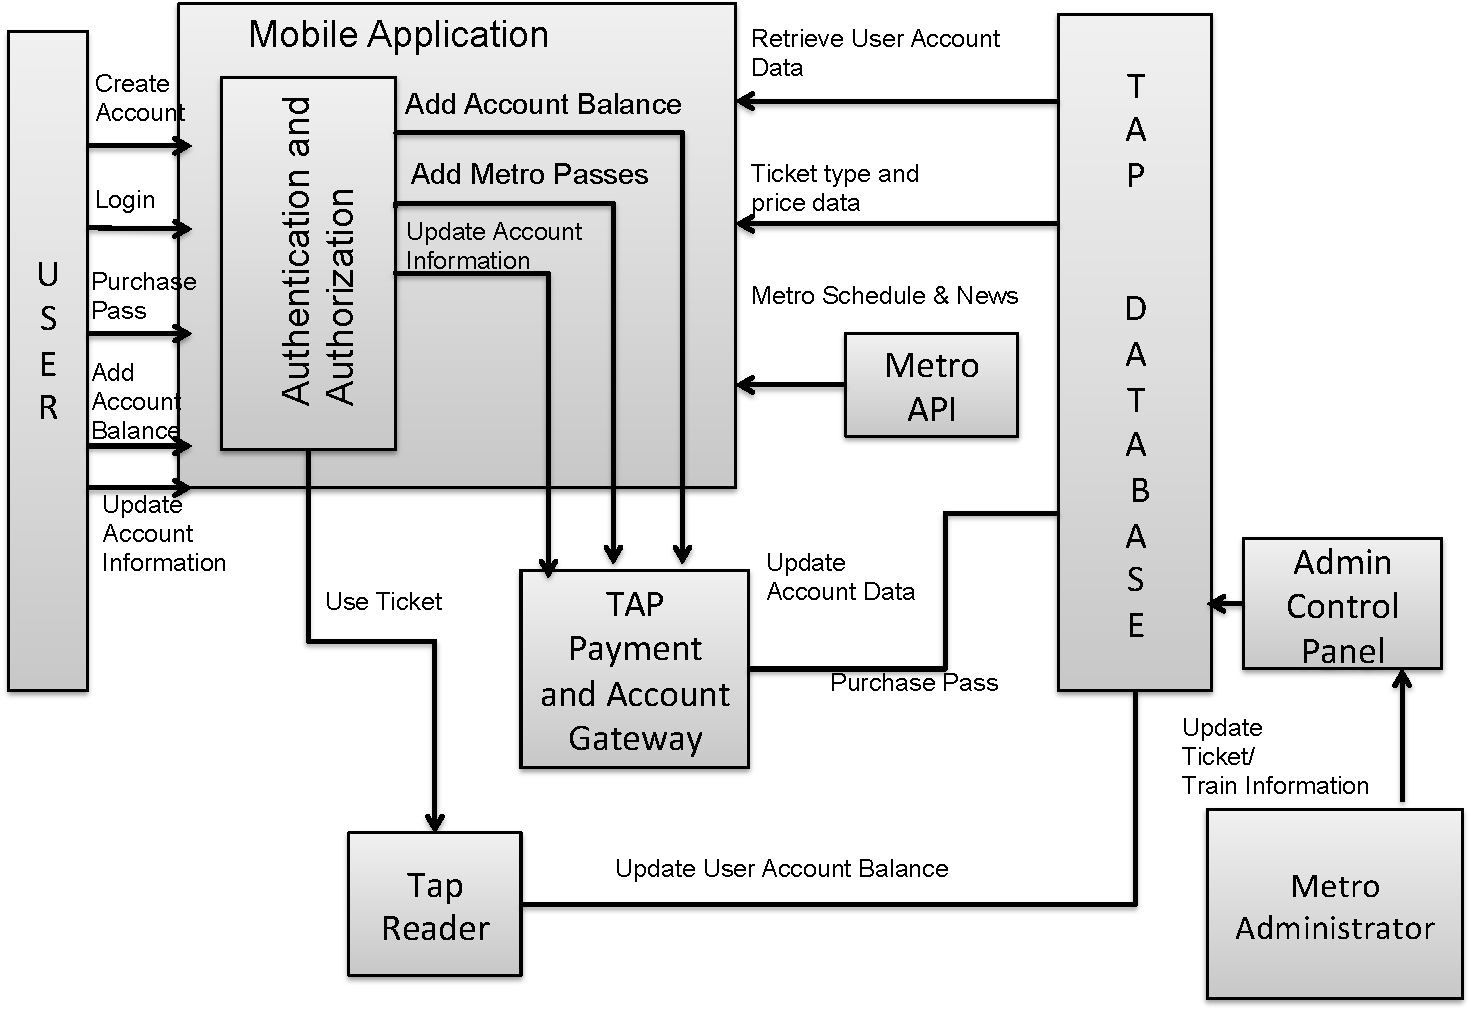
\includegraphics[width=\textwidth]{OCD/element-relationship.pdf}
		\end{figure}			

\clearpage
	\subsubsection{Proposed Workflow}
		\begin{figure}[!htbp]
			\centering
			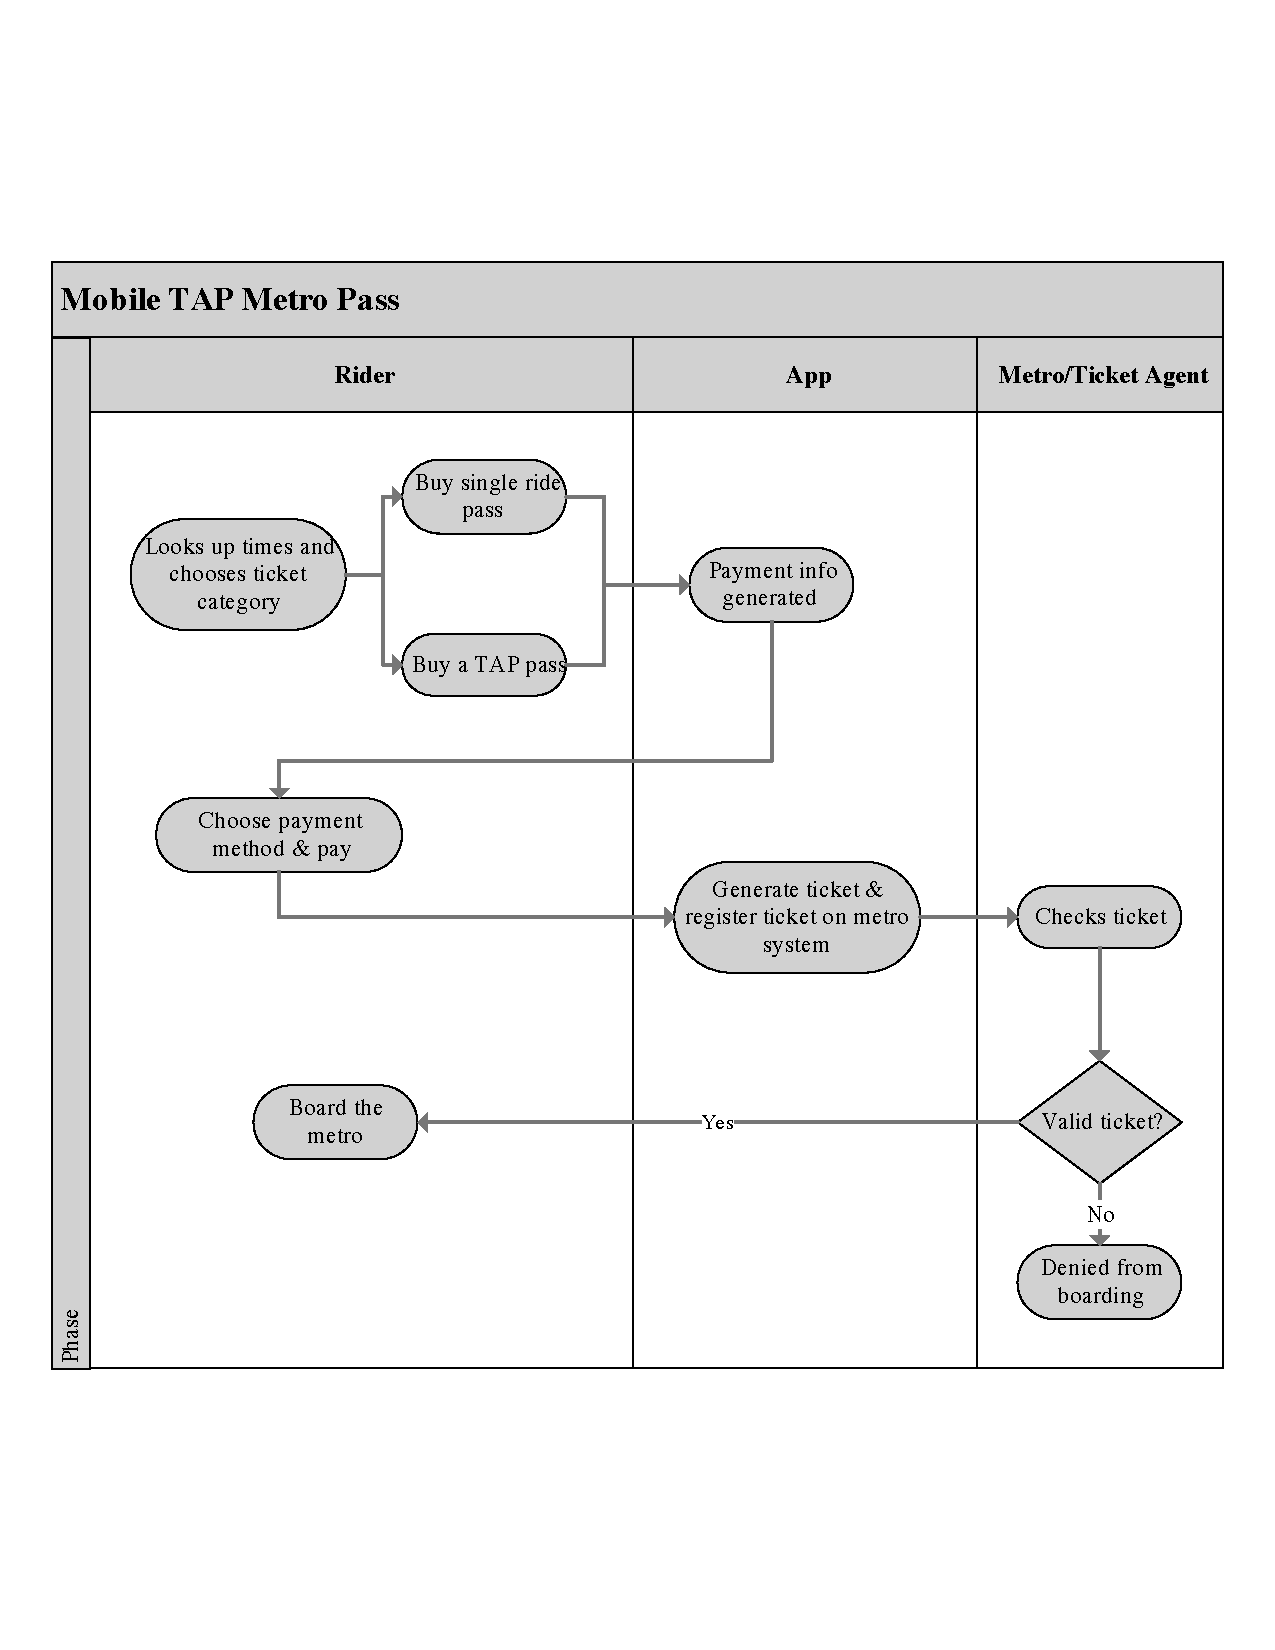
\includegraphics[width=\textwidth]{OCD/uml.pdf}
		\end{figure}
	
\newpage
\section{Requirements}
\subsection{Capability Requirements}

	\subsubsection{Platform}\begin{enumerate}
		\item The application shall be compatible with the iOS and Android mobile platforms.
		\item The application shall support a web interface for other mobile devices.
	\end{enumerate}
	
	\subsubsection{User Accounts}\begin{enumerate}
		\item If it is a user’s first-time opening the application, the application shall prompt the user to enter an email address, password, and credit card information.
		\begin{enumerate}
			\item If the account is created successfully, the application shall send a confirmation to the user’s stored email address.
			\item If the account creation is not successful, the application shall display an error message that prompts the user to reenter their information and will not be logged in.
		\end{enumerate}
		\item If a returning user opens the application, it shall prompt the user to enter their log-in information.
			\begin{enumerate}
				\item If the log-in attempt fails, the application will display an error message that prompts the user to reenter their log-in information.
				\item If the log-in attempt succeeds, the user will be shown a transit management screen.
			\end{enumerate}
	\end{enumerate}
	
	\subsubsection{Usage}\begin{enumerate}
		\item If the application loses connectivity, the application shall display an error message. 
		\item The application shall retrieve the user’s location at intervals of $120\pm10$ seconds.
		\item If the user is within 150 feet of a train-stop’s geo-location coordinates, the train-stop’s name, ticket price, and incoming train information shall be displayed on the user interface.
		\item If train stop information is being displayed on the application’s user interface, the application shall update the train stop’s incoming train information at intervals of $30\pm 5$ seconds.
	\end{enumerate}
	
	\subsubsection{Payments}\begin{enumerate}
		\item If the user selects to purchase a ticket, their stored credit card will be charged for the price of the train stop’s ticket.
		\begin{enumerate}
			\item If the card does not process, an error message shall by display and the order shall not be accepted.
			\item If the transaction succeeds, the application shall create a virtual ticket.
		\end{enumerate}
		\item If the user selects to use their ticket, the application shall signal the gate up to a maximum of 3 attempts at $20\pm 5$ second intervals to open.
			\begin{enumerate}
				\item If the application is unsuccessful on the 3rd attempt, an error message shall be displayed.
				\item Otherwise, the turnstile is unlocked, permitting the user to pass through.
			\end{enumerate}
		\item The application shall store unused virtual tickets for at least 1 year.
		\item The application shall store used virtual tickets for at least 30 days.
		\item The application shall allow the user to change their email address.
		\item The application shall allow the user to change their password.
		\item The application shall allow the user to change their credit card information.
	\end{enumerate}		
\newpage	
\subsection{Level of Service Requirements}

\begin{table}[h]
    \begin{tabularx}{\textwidth}{Xll}
    \hline
    LOS Requirements                                                                                          & Desired Level & Accepted Level \\ \hline
    LOS-1: Concurrent Users                                                                                   & $150000$         & $75000$           \\
    LOS-2: Start-up and user location time                                                                    & 7             & 15             \\
    LOS-3: Ticket Purchase Transaction Time                                                                   & 5             & 20             \\
    LOS-4: Update Account Information Time                                                                    & 10            & 30             \\
    LOS-5: Tickets stored per user                                                                            & 1500          & 500            \\
    LOS-6: \% first-time users able to purchase ticket without outside help                                    & 99            & 95             \\
    LOS-7: \% first-time users able to use ticket without outside help                                         & 99            & 95             \\
    LOS-8: \% users that ride metro at least once per week that would rate ease of use at 3 out of 5 or higher & 80            & 75             \\
    LOS-9: Average Time for User to Create an Account                                                         & 45            & 60             \\
    LOS-10: Failed Ticket Purchases per 1000                                                                  & 1             & 5              \\
    LOS-11: Failed Ticket Uses per 1000                                                                       & 1             & 5              \\
    LOS-12: Hours per day that app shall purchase tickets                                                     & 22            & 20             \\
    LOS-13: Hours per day that app shall allow use of tickets                                                 & 22            & 20             \\
    LOS-14: \# iOS generations app shall support                                                               & 3             & 2              \\
    LOS-15: \# Android generations app shall support                                                           & 3             & 2              \\
    LOS-16: \# versions of app that Metro system shall support                                                 & 3             & 2              \\
    \hline
    \end{tabularx}
\end{table}
\newpage
\newcommand{\risk}[5]{
	\rule{\textwidth}{.1pt}
	\textbf{ Risk\# #1}(Last week: #2)\\
	\textbf{Weeks Active} #3
	\paragraph{Risk Description} #4
	\paragraph{Mitigation Action Items} #5\\
}

\section{Risk Lists}

\subsection{Technical Risks}

\risk{1}{N/A}{1}{
An unsecure platform might be exploited or easily manipulated (e.g. people finding loopholes to avoid fees), which can result in the LA Metro losing profits.
}{
Our group’s architect will develop a cryptosystem for our application that will be tested until it meets the client’s requirements and security standards.
}
\risk{3}{N/A}{1}{
A technical malfunction of our platform might cause boarding delays for passengers and cause inefficiencies in LA Metro operations.
}{
A back-up system will be designed in a later stage of the project. Also, we will advise passengers who are particularly sensitive to delays to have a back-up physical tap card.
}
\risk{4}{N/A}{1}{
End users (passengers) might not have smartphones that have the technical capabilities to support our platform.
}{
A feasibility study will be conducted to verify compatible phone penetration rates, and if needed, we can tailor our platform to target only a certain segment of the customer base that has access to the required technology.
}
\risk{8}{N/A}{1}{
We will be using PhoneGap to implement the mobile application with standard web technologies like HTML/CSS/Javascript which makes the application subject to device-specific mobile browser display discrepencies.
}{
Test on a wide variety of devices (different iPhone versions and various Android phones) to ensure the application is rendered properly on all screen sizes and OS versions.
}

\subsection{Requirement Risks}
\risk{2}{N/A}{1}{
The LA Metro might not be willing to implement our system or work with our group to test our platform on their systems/hardware.
}{
Our project manager is currently in talks with the LA Metro authorities, but we could also potentially do a proof of concept using similar hardware/systems.
}
\risk{6}{N/A}{1}{
After the platform has been implemented and integrated, the LA Metro requirements might change, or the technologies being used in relevant processes might change.
}{
If we are under a contract/agreement, the team will develop updates/patches that will adapt to new requirements. Otherwise, we will give the LA Metro a copy of our comprehensive documentation for the software so that necessary changes can be handled in-house.
}
\risk{5}{N/A}{1}{
To get the application fully working and integrated into the LA Metro system, there will be a large set of evolving requirements. Two semesters might not be enough time to complete the project, especially if there are unexpected risks (e.g. another developer completes the same project before we do, bureaucratic risks, etc.)
}{
We will develop a running list of unexpected risks as they come up and develop strategies to approach them. For example, we would explicitly ask LA Metro for their timeline and ask for an exclusive partnership.
}

\subsection{Human Resources Risks}

\risk{7}{N/A}{1}{
Due to rapid formation of teams without proper analysis of required skill sets needed for this project we may lack the technical skills to complete this project in a professionally acceptable manner.
}{
Identify team member skills and project requirements so we can individually prepare ourselves for technologies that we will be implementing next semester.
}
\risk{9}{N/A}{1}{
The statically defined list of team roles may not fit our specific project requirements.
}{
Dynamically reassign team roles as the project and its requirements mature.  Also the team shall be aware that responsibilities will be very flexible and we may need to step outside the scope of our assigned position
}
\risk{10}{N/A}{1}{
The amount of cooperation needed between our team and LA Metro may be more than expected which could make this project unfeasible for them.
}{
Come up with a plan focused around the idea that LA Metro should have to do as little as possible.  Extensive testing should be done internally before our software can be ready for LA Metro.  The goal should be to get it right the first time.
}
\rule{\textwidth}{.1pt}
%\begin{landscape}
%\begin{table}[h]
\begin{center}
\begin{tabularx}{\textwidth}{cccXXc}

1 & N/A & Security & An unsecure platform might be exploited or easily manipulated (e.g. people finding loopholes to avoid fees), which can result in the LA Metro losing profits. & Our group�s architect will develop a cryptosystem for our application that will be tested until it meets the client�s requirements and security standards. & 1 \\ 
2 & N/A & Partnership & The LA Metro might not be willing to implement our system or work with our group to test our platform on their systems/hardware. & Our project manager is currently in talks with the LA Metro authorities, but we could also potentially do a proof of concept using similar hardware/systems. & 1 \\ 
3 & N/A & Technology & A technical malfunction of our platform might cause boarding delays for passengers and cause inefficiencies in LA Metro operations. & A back-up system will be designed in a later stage of the project. Also, we will advise passengers who are particularly sensitive to delays to have a back-up physical tap card. & 1 \\ 
4 & N/A & Technology & End users (passengers) might not have smartphones that have the technical capabilities to support our platform. & A feasibility study will be conducted to verify compatible phone penetration rates, and if needed, we can tailor our platform to target only a certain segment of the customer base that has access to the required technology. & 1 \\ 
5 & N/A & Estimation & To get the application fully working and integrated into the LA Metro system, there will be a large set of evolving requirements. Two semesters might not be enough time to complete the project, especially if there are unexpected risks (e.g. another developer completes the same project before we do, bureaucratic risks, etc.) & We will develop a running list of unexpected risks as they come up and develop strategies to approach them. For example, we would explicitly ask LA Metro for their timeline and ask for an exclusive partnership. & 1 \\ 
6 & N/A & Requirements & After the platform has been implemented and integrated, the LA Metro requirements might change, or the technologies being used in relevant processes might change. & If we are under a contract/agreement, the team will develop updates/patches that will adapt to new requirements. Otherwise, we will give the LA Metro a copy of our comprehensive documentation for the software so that necessary changes can be handled in-house. & 1 \\ 
7 & N/A & People & Due to rapid formation of teams without proper analysis of required skill sets needed for this project we may lack the technical skills to complete this project in a professionally acceptable manner.
 & Identify team member skills and project requirements so we can individually prepare ourselves for technologies that we will be implementing next semester. & 1 \\ 
8 & N/A & Tools & We will be using PhoneGap to implement the mobile application with standard web technologies like HTML/CSS/Javascript which makes the application subject to device-specific mobile browser display discrepencies. & Test on a wide variety of devices (different iPhone versions and various Android phones) to ensure the application is rendered properly on all screen sizes and OS versions. & 1 \\ 
9 & N/A & Organizational & The statically defined list of team roles may not fit our specific project requirements. & Dynamically reassign team roles as the project and its requirements mature.  Also the team shall be aware that responsibilities will be very flexible and we may need to step outside the scope of our assigned position & 1 \\ 
10 & N/A & Estimation & The amount of cooperation needed between our team and LA Metro may be more than expected which could make this project unfeasible for them. & Come up with a plan focused around the idea that LA Metro should have to do as little as possible.  Extensive testing should be done internally before our software can be ready for LA Metro.  The goal should be to get it right the first time. & 1 \\ 
\end{tabularx}
\end{center}
\end{table}

%\end{landscape}

		
\end{document}